
\chapter{Risultati e discussioni}
\fancyhead[RO]{\bfseries Risultati e discussioni}

\section{Difficoltà e problematiche riscontrate}

Nello sviluppo del progetto sono state riscontrate varie problematiche, dovute anche ai limiti del software e dell'hardware utilizzato.


\subsection{Lo studio delle trasformazioni}
Lo studio condotto per arrivare a formulare il metodo usato per creare le giuste trasformazioni, ha occupato diverse giornate di lavoro, all'incirca una trentina.

Infatti, dopo aver studiato le basi delle trasformazioni, queste sono state sviluppate procedendo sia per ragionamenti dovuti a calcoli preliminari, sia per tentativi empirici. Fare prove inserendo valori casuali nelle varie operazioni è stato d'aiuto, in effetti, per comprendere meglio le variazioni del comportamento del sistema. Una volta trovata la trasformazione corretta, tuttavia, si è continuato a fare ulteriori prove, in quanto non tutto era ancora ben chiaro. Questo è stato utile a comprendere quando la trasformazione funzionasse, o meglio, a stabilire le condizioni necessarie per produrre l'effetto desiderato, e quindi rendere la trasformazione efficace.


\subsection{I limiti dell'hardware}
L'obiettivo del progetto era quello di creare un'applicazione usufruibile da ogni utente, disponendo solamente di un pc e una webcam. Tuttavia si è notato che la qualità dell'hardware incide nella resa dell'applicazione.

Le prime prove sono state fatte utilizzando le coordinate del mouse, al posto delle coordinate del volto rilevato. Si è notato che, importando il modulo OpenCV, la velocità di esecuzione veniva fortemente rallentata, perché il solo rilevamento è un processo molto dispendioso. Aggiungendo il carico di lavoro dovuto alla parte grafica, il risultato era inaccettabile, renderizzando circa 15 frames al secondo (utilizzando un processore Intel I5 e una scheda grafica ATI Radeon HD 5650, quindi hardware di qualità medio-alta).

Fortunatamente esiste un parametro, nella funzione \textit{detect\_multi\_scale()} situato nel modulo OpenCV, che ha permesso di migliorare la velocità senza diminuire la qualità. Questo parametro era relativo alle dimensioni dell'area minima da analizzare per il rilevamento; più è piccola l'area e più calcoli deve eseguire l'algoritmo per riconoscere i volti. All'inizio era impostato a $(30,30)$, in questo modo i volti venivano ricercati in aree di minimo 30 pixel per 30. Aumentanto questo valore a circa $(100,100)$, la velocità di esecuzione è stata portata a 30 frames al secondo, utilizzando anche scene complesse, in cui erano presenti alcune centinaia di migliaia di vertici. Questi valori permettono, utilizzando una webcam di risoluzione $640\times480$, di rilevare volti fino ad una distanza di circa un metro e mezzo dallo schermo, perciò il compromesso è accettabile.

La qualità della webcam può incidere nella facilitazione del riconoscimento, permettendo di elaborare immagini migliori, e quindi diminuire il rumore generato dall'imprecisione del rilevamento. Tuttavia, aumentando la risoluzione della webcam, la velocità può essere compromessa, in quanto i frames, che OpenCV deve analizzare, hanno dimensioni più elevate, perciò devono essere  eseguiti più calcoli.

Allo stesso modo può influire l'angolo di apertura della webcam: più l'angolo è ampio e meglio si può apprezzare l'illusione, in quanto l'utente ha più spazio per potersi muovere senza essere perso dall'obiettivo della webcam, causando interruzioni nella trasformazione. 

\subsection{I limiti di OpenCV}

Come è stato già accennato, OpenCV fornisce dei metodi che hanno delle limitazioni: il rilevamento non è preciso, e genera sempre una sorta di oscillamento nelle coordinate rilevate durante il tracking, inoltre non è in grado di stimare la distanza dallo schermo.

Per quanto riguarda il primo limite si può dire che, grazie all'aggiunta dell'algoritmo che funge da filtro, il problema è stato risolto senza incidere troppo sulla qualità finale.

Per quanto riguarda il secondo limite, invece, il risultato sperato non è stato raggiunto. Per ottenere un effetto più realistico, infatti, la trasformazione dovrebbe tenere conto in modo preciso della distanza dell'utente, poiché le coordinate $x$ e $y$ della telecamera virtuale andrebbero calcolate anche in funzione di essa. Questo è dovuto al fatto che anche la webcam possiede un proprio frustum, e quindi spostamenti lungo l'asse X o Y non rimangono proporzionati al variare della distanza, ovvero della coordinata $z$. Infatti, all'aumentare della distanza dallo schermo, gli spostamenti rilevati lungo gli assi X e Y variano più lentamente, di conseguenza la prospettiva sarà trasformata più lentamente.

Il calcolo della distanza non è banale con una semplice webcam. Bisognerebbe effettuare una calibrazione ad ogni esecuzione per misurare la grandezza della testa dell'utente in modo da trovare un coefficiente per ricalcolare la $x$ e la $y$. Poiché anche il rilevamento non è preciso e varia in base a molti fattori, questa caratteristica richiede uno studio molto approfondito, e un gran numero di prove.

Il problema potrebbe essere risolto utilizzando un sensore apposito, come il Kinect della Microsoft, che stima in modo abbastanza preciso le distanze grazie a raggi infrarossi, ma questo andrebbe contro la logica dell'applicazione, che mira ad offrire questa forma di interazione utilizzando semplicemente una webcam.

\subsection{Importazione modelli in OpenGL}
In OpenGL è stato riscontrato un problema nell'importazione dei modelli 3D con estensione .obj. Infatti, quando erano renderizzati a schermo, risultava che la trasformazione che essi subivano fosse ritardata di uno o due frames rispetto agli altri oggetti disegnati direttamente in OpenGL. Questo generava un'irregolarità nel movimento apparente degli oggetti, producendo un'effetto simile ad una sorta di tremolio.

Il difetto probabilmente era legato ai driver della scheda grafica, tuttavia non sono state fatte prove su altre macchine quindi il problema è rimasto irrisolto.

Successivamente, lo sviluppo è passato ad Ogre3D, che permette di gestire più efficientemente scene importate dall'esterno, perciò la parte OpenGL è stata messa da parte. Con Ogre3D il problema non è ricomparso.



\section{I requisiti dell'applicazione}
In questa sezione riassumiamo le condizioni che devono essere rispettate per una miglior resa dell'applicazione:

\begin{itemize}
\item \textit{Ambiente}: L'ambiente in cui si usa l'applicazione deve essere ben illuminato, per facilitare il riconoscimento del volto. La scarsa illuminazione, rendendo più faticoso il rilevamento, causa una caduta di prestazioni in termini di velocità di esecuzione.

Inoltre lo spazio intorno all'utente dovrebbe essere libero da cose che possono creare interferenze o falsi positivi (altre persone, magliette, disegni o poster raffiguranti volti, etc).

\item \textit{Webcam}: La webcam dovrebbe essere di buona qualità, ma con una risoluzione non troppo alta, per evitare che le dimensioni dei frames rendano il rilevamento troppo complesso\footnote{In caso di utilizzo di hardware di media o bassa qualità}.

Inoltre la webcam deve essere posizionata sopra lo schermo, al centro, cioè nella posizione di default dei computer portatili, altrimenti la prospettiva dell'utente non sarebbe allineata con quella della telecamera virtuale.

\item \textit{Scena 3D}: Per rendere l'illusione più efficace\footnote{Come è stato già detto, la trasformazione è corretta anche se la scena non rispetta queste condizioni}, la scena 3D importata dovrebbe essere racchiusa in un box di dimensioni uguali a quelle del frustum, con l'apertura giacente sul near plane. Inoltre l'aspect ratio del box dovrebbe rispettare quella dello schemo, per evitare stiramenti o rimpicciolimenti della scena.

Nel progetto sviluppato in Ogre3D è stato aggiunto un file di configurazione, dove l'utente può specificare le coordinate dei punti che identificano il suo box. Tramite queste coordinate il programma imposta le dimensioni del frustum e trasla la scena centrandola nell'origine, allineandola così con il frustum. 

Impostando i valori giusti, l'apertura del box rimane coincidente con lo schermo (quando si usa lo schermo intero), e, durante la trasformazione di prospettiva, i bordi rimangono allineati, creando l'illusione che lo schermo abbia una profondità.
\end{itemize}

\section{Risultati}
Nel corso dello sviluppo del progetto sono stati apportati notevoli miglioramenti nel funzionamento dell'applicazione. Essa è stata provata da alcuni utenti (familiari e conoscenti), e tutti sono rimasti affascinati dall'effetto prodotto. Arrivati al punto attuale, perciò, si può dire che i risultati sono accettabili, in quanto l'illusione che si voleva creare è più che apprezzabile.

Nelle seguenti immagini è possibile vedere il corretto funzionamento dell'applicazione.

\begin{figure}[htbp]
\centering
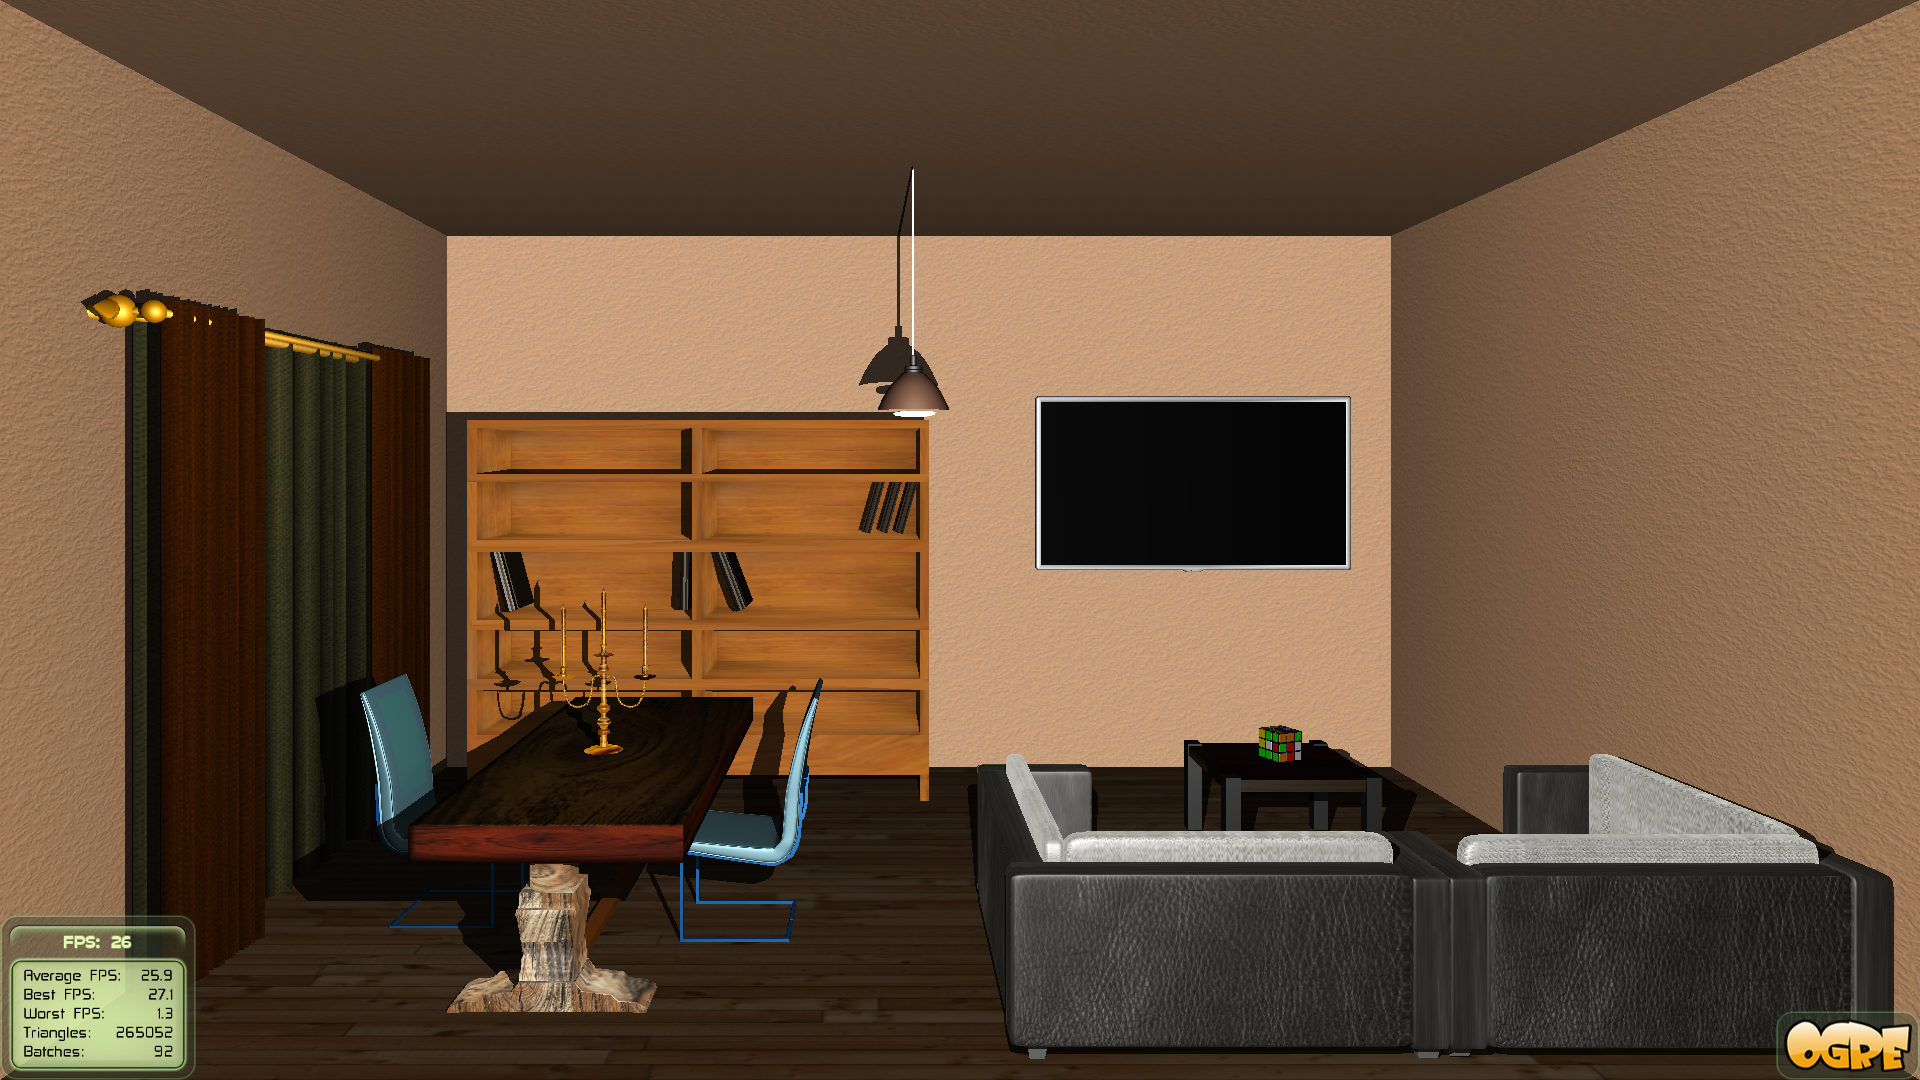
\includegraphics[width=0.8\textwidth]{images/progetto/ogre.png}
\caption{Scena vista frontalmente.\label{liv-room}}
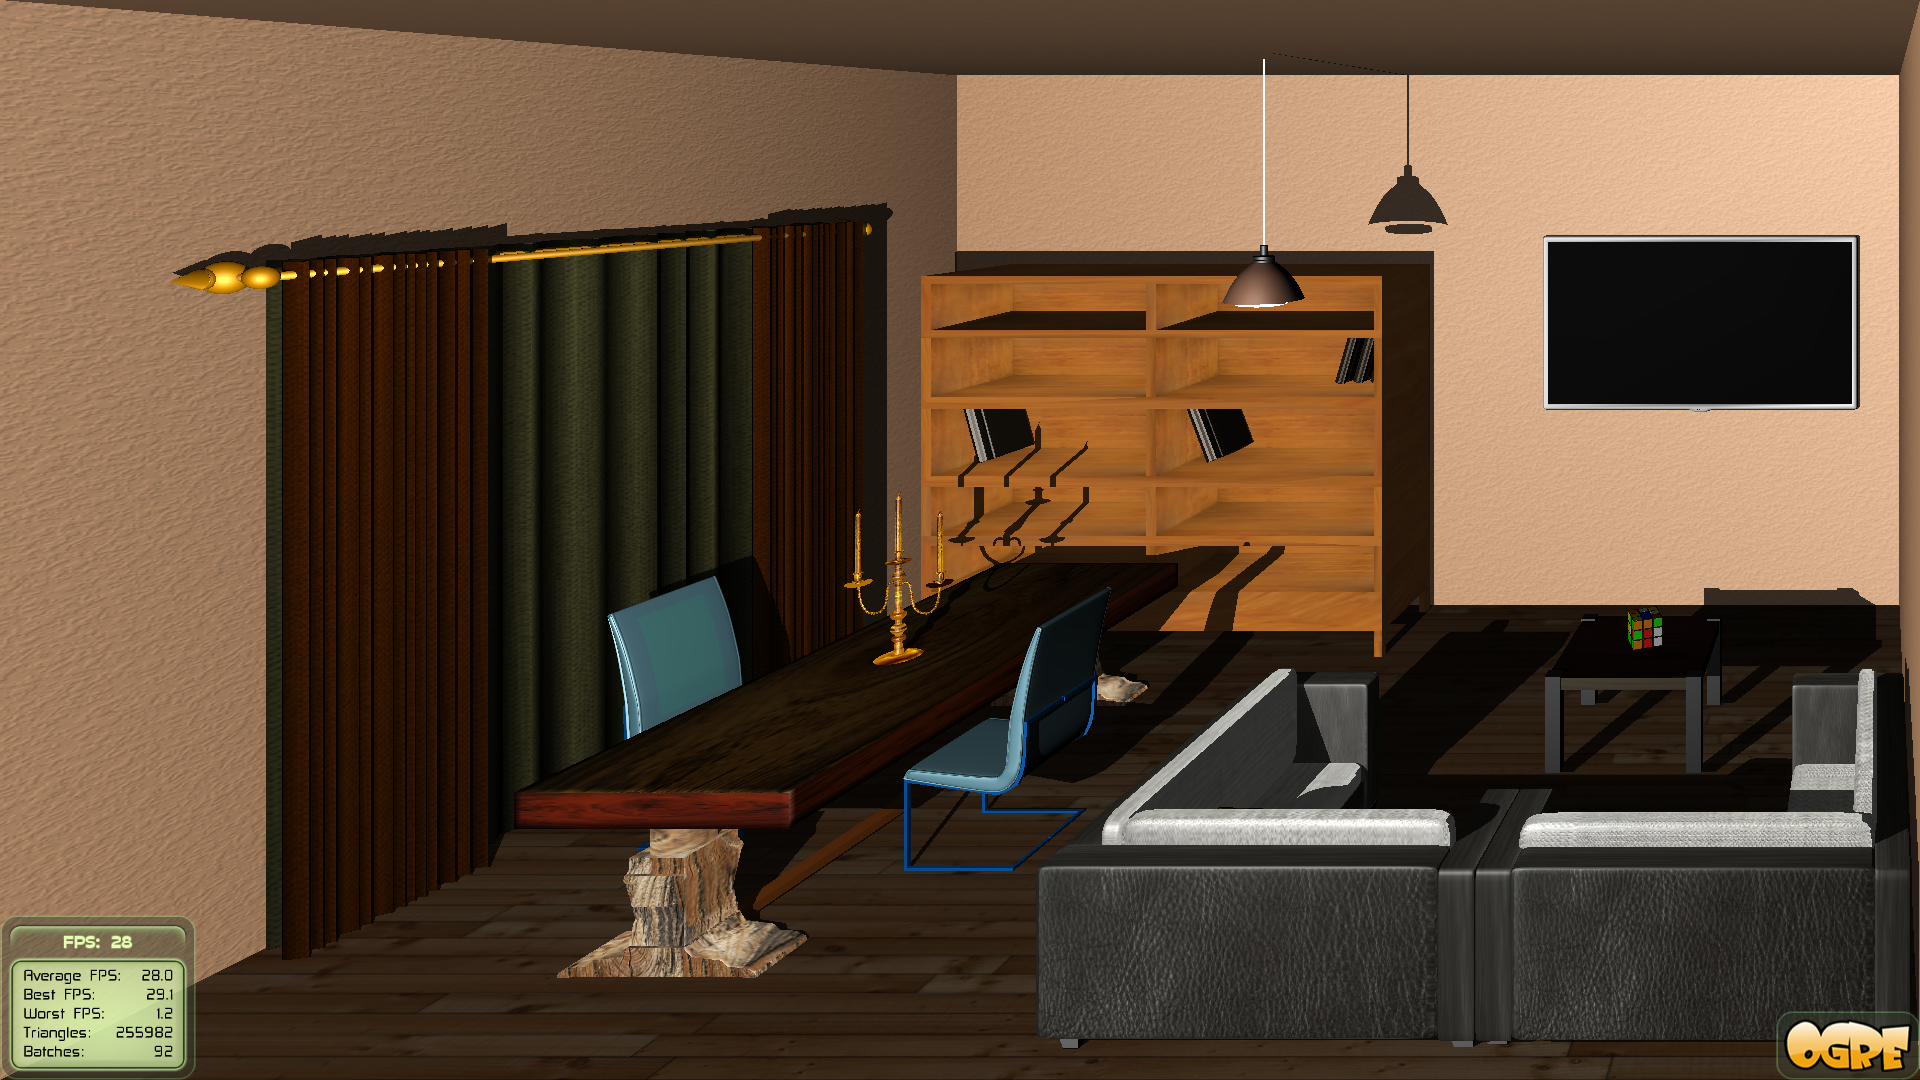
\includegraphics[width=0.8\textwidth]{images/progetto/ogre-2.png}
\caption{Prospettiva modificata in seguito ad uno spostamento dell'utente verso l'alto a destra.\label{liv-room}}
\end{figure}
\clearpage
